\documentclass[12pt,a4paper]{article}

\usepackage[rmargin=1.2in,lmargin=1.2in,tmargin=.8in,bmargin=.8in]{geometry}
\usepackage{indentfirst}

% fonts
% \usepackage{mathptmx}
\usepackage{fontspec}
\setmainfont{Times New Roman}

% images, table and colors
\usepackage[dvipsnames]{xcolor}
\usepackage{graphicx} 
\graphicspath{ {./figures/}, {/Users/luducheng/Documents/templates/logos/OBSPM/LERMA/RGB - RVB/Noir/}} 
\usepackage{tabularx, makecell}
\usepackage{caption}
\usepackage{subcaption}
\usepackage{enumitem}
\usepackage[normalem]{ulem}

% math support
\usepackage{amsmath}
\usepackage{amssymb,stackengine}
\newcommand\varlesssim{\mathrel{\ensurestackMath{%
  \stackengine{-.4ex}{<}{\rotatebox{-25}{$\sim$}}{U}{r}{F}{T}{S}}}}
\newcommand\vargtrsim{\mathrel{\ensurestackMath{%
  \stackengine{-.4ex}{>}{\rotatebox{25}{$\sim$}}{U}{l}{F}{T}{S}}}}
\usepackage{siunitx}
\DeclareSIUnit{\erg}{erg}
\DeclareSIUnit{\rate}{\erg \per \centi \metre \cubed \per \second}
\usepackage[version=4]{mhchem}

% for code display
\usepackage{minted}

% citations
\usepackage[colorlinks=true,allcolors=blue]{hyperref}
\usepackage[backend=biber, citestyle=authoryear-icomp,bibstyle=authoryear,hyperref=true,isbn=false,url=false,eprint=false,date=year,maxcitenames=2,uniquelist=minyear,sorting=ynt]{biblatex}
\addbibresource{./pdr_references.bib}
%
%  These Macros are taken from the AAS TeX macro package version 5.2
%  and are compatible with the macros in the A&A document class
%  version 7.0
%  Include this file in your LaTeX source only if you are not using
%  the AAS TeX macro package or the A&A document class and need to
%  resolve the macro definitions in the TeX/BibTeX entries returned by
%  the ADS abstract service.
%
%  If you plan not to use this file to resolve the journal macros
%  rather than the whole AAS TeX macro package, you should save the
%  file as ``aas_macros.sty'' and then include it in your LaTeX paper
%  by using a construct such as:
%	\documentstyle[11pt,aas_macros]{article}
%
%  For more information on the AASTeX and A&A packages, please see:
%       http://journals.aas.org/authors/aastex.html	
%       ftp://ftp.edpsciences.org/pub/aa/readme.html
%  For more information about ADS abstract server, please see:
%       http://adsabs.harvard.edu/ads_abstracts.html
%

% Abbreviations for journals.  The object here is to provide authors
% with convenient shorthands for the most "popular" (often-cited)
% journals; the author can use these markup tags without being concerned
% about the exact form of the journal abbreviation, or its formatting.
% It is up to the keeper of the macros to make sure the macros expand
% to the proper text.  If macro package writers agree to all use the
% same TeX command name, authors only have to remember one thing, and
% the style file will take care of editorial preferences.  This also
% applies when a single journal decides to revamp its abbreviating
% scheme, as happened with the ApJ (Abt 1991).

\makeatletter
\let\jnl@style=\rm
\def\ref@jnl#1{{\jnl@style#1}}

\def\aj{\ref@jnl{AJ}}                   % Astronomical Journal
\def\actaa{\ref@jnl{Acta Astron.}}      % Acta Astronomica
\def\araa{\ref@jnl{ARA\&A}}             % Annual Review of Astron and Astrophys
\def\apj{\ref@jnl{ApJ}}                 % Astrophysical Journal
\def\apjl{\ref@jnl{ApJ}}                % Astrophysical Journal, Letters
\def\apjs{\ref@jnl{ApJS}}               % Astrophysical Journal, Supplement
\def\ao{\ref@jnl{Appl.~Opt.}}           % Applied Optics
\def\apss{\ref@jnl{Ap\&SS}}             % Astrophysics and Space Science
\def\aap{\ref@jnl{A\&A}}                % Astronomy and Astrophysics
\def\aapr{\ref@jnl{A\&A~Rev.}}          % Astronomy and Astrophysics Reviews
\def\aaps{\ref@jnl{A\&AS}}              % Astronomy and Astrophysics, Supplement
\def\azh{\ref@jnl{AZh}}                 % Astronomicheskii Zhurnal
\def\baas{\ref@jnl{BAAS}}               % Bulletin of the AAS
\def\bac{\ref@jnl{Bull. astr. Inst. Czechosl.}}
                % Bulletin of the Astronomical Institutes of Czechoslovakia 
\def\caa{\ref@jnl{Chinese Astron. Astrophys.}}
                % Chinese Astronomy and Astrophysics
\def\cjaa{\ref@jnl{Chinese J. Astron. Astrophys.}}
                % Chinese Journal of Astronomy and Astrophysics
\def\icarus{\ref@jnl{Icarus}}           % Icarus
\def\jcap{\ref@jnl{J. Cosmology Astropart. Phys.}}
                % Journal of Cosmology and Astroparticle Physics
\def\jrasc{\ref@jnl{JRASC}}             % Journal of the RAS of Canada
\def\memras{\ref@jnl{MmRAS}}            % Memoirs of the RAS
\def\mnras{\ref@jnl{MNRAS}}             % Monthly Notices of the RAS
\def\na{\ref@jnl{New A}}                % New Astronomy
\def\nar{\ref@jnl{New A Rev.}}          % New Astronomy Review
\def\pra{\ref@jnl{Phys.~Rev.~A}}        % Physical Review A: General Physics
\def\prb{\ref@jnl{Phys.~Rev.~B}}        % Physical Review B: Solid State
\def\prc{\ref@jnl{Phys.~Rev.~C}}        % Physical Review C
\def\prd{\ref@jnl{Phys.~Rev.~D}}        % Physical Review D
\def\pre{\ref@jnl{Phys.~Rev.~E}}        % Physical Review E
\def\prl{\ref@jnl{Phys.~Rev.~Lett.}}    % Physical Review Letters
\def\pasa{\ref@jnl{PASA}}               % Publications of the Astron. Soc. of Australia
\def\pasp{\ref@jnl{PASP}}               % Publications of the ASP
\def\pasj{\ref@jnl{PASJ}}               % Publications of the ASJ
\def\rmxaa{\ref@jnl{Rev. Mexicana Astron. Astrofis.}}%
                % Revista Mexicana de Astronomia y Astrofisica
\def\qjras{\ref@jnl{QJRAS}}             % Quarterly Journal of the RAS
\def\skytel{\ref@jnl{S\&T}}             % Sky and Telescope
\def\solphys{\ref@jnl{Sol.~Phys.}}      % Solar Physics
\def\sovast{\ref@jnl{Soviet~Ast.}}      % Soviet Astronomy
\def\ssr{\ref@jnl{Space~Sci.~Rev.}}     % Space Science Reviews
\def\zap{\ref@jnl{ZAp}}                 % Zeitschrift fuer Astrophysik
\def\nat{\ref@jnl{Nature}}              % Nature
\def\iaucirc{\ref@jnl{IAU~Circ.}}       % IAU Cirulars
\def\aplett{\ref@jnl{Astrophys.~Lett.}} % Astrophysics Letters
\def\apspr{\ref@jnl{Astrophys.~Space~Phys.~Res.}}
                % Astrophysics Space Physics Research
\def\bain{\ref@jnl{Bull.~Astron.~Inst.~Netherlands}} 
                % Bulletin Astronomical Institute of the Netherlands
\def\fcp{\ref@jnl{Fund.~Cosmic~Phys.}}  % Fundamental Cosmic Physics
\def\gca{\ref@jnl{Geochim.~Cosmochim.~Acta}}   % Geochimica Cosmochimica Acta
\def\grl{\ref@jnl{Geophys.~Res.~Lett.}} % Geophysics Research Letters
\def\jcp{\ref@jnl{J.~Chem.~Phys.}}      % Journal of Chemical Physics
\def\jgr{\ref@jnl{J.~Geophys.~Res.}}    % Journal of Geophysics Research
\def\jqsrt{\ref@jnl{J.~Quant.~Spec.~Radiat.~Transf.}}
                % Journal of Quantitiative Spectroscopy and Radiative Transfer
\def\memsai{\ref@jnl{Mem.~Soc.~Astron.~Italiana}}
                % Mem. Societa Astronomica Italiana
\def\nphysa{\ref@jnl{Nucl.~Phys.~A}}   % Nuclear Physics A
\def\physrep{\ref@jnl{Phys.~Rep.}}   % Physics Reports
\def\physscr{\ref@jnl{Phys.~Scr}}   % Physica Scripta
\def\planss{\ref@jnl{Planet.~Space~Sci.}}   % Planetary Space Science
\def\procspie{\ref@jnl{Proc.~SPIE}}   % Proceedings of the SPIE

\let\astap=\aap
\let\apjlett=\apjl
\let\apjsupp=\apjs
\let\applopt=\ao
\makeatother % to compile on my computer
% %
%  These Macros are taken from the AAS TeX macro package version 5.2
%  and are compatible with the macros in the A&A document class
%  version 7.0
%  Include this file in your LaTeX source only if you are not using
%  the AAS TeX macro package or the A&A document class and need to
%  resolve the macro definitions in the TeX/BibTeX entries returned by
%  the ADS abstract service.
%
%  If you plan not to use this file to resolve the journal macros
%  rather than the whole AAS TeX macro package, you should save the
%  file as ``aas_macros.sty'' and then include it in your LaTeX paper
%  by using a construct such as:
%	\documentstyle[11pt,aas_macros]{article}
%
%  For more information on the AASTeX and A&A packages, please see:
%       http://journals.aas.org/authors/aastex.html	
%       ftp://ftp.edpsciences.org/pub/aa/readme.html
%  For more information about ADS abstract server, please see:
%       http://adsabs.harvard.edu/ads_abstracts.html
%

% Abbreviations for journals.  The object here is to provide authors
% with convenient shorthands for the most "popular" (often-cited)
% journals; the author can use these markup tags without being concerned
% about the exact form of the journal abbreviation, or its formatting.
% It is up to the keeper of the macros to make sure the macros expand
% to the proper text.  If macro package writers agree to all use the
% same TeX command name, authors only have to remember one thing, and
% the style file will take care of editorial preferences.  This also
% applies when a single journal decides to revamp its abbreviating
% scheme, as happened with the ApJ (Abt 1991).

\makeatletter
\let\jnl@style=\rm
\def\ref@jnl#1{{\jnl@style#1}}

\def\aj{\ref@jnl{AJ}}                   % Astronomical Journal
\def\actaa{\ref@jnl{Acta Astron.}}      % Acta Astronomica
\def\araa{\ref@jnl{ARA\&A}}             % Annual Review of Astron and Astrophys
\def\apj{\ref@jnl{ApJ}}                 % Astrophysical Journal
\def\apjl{\ref@jnl{ApJ}}                % Astrophysical Journal, Letters
\def\apjs{\ref@jnl{ApJS}}               % Astrophysical Journal, Supplement
\def\ao{\ref@jnl{Appl.~Opt.}}           % Applied Optics
\def\apss{\ref@jnl{Ap\&SS}}             % Astrophysics and Space Science
\def\aap{\ref@jnl{A\&A}}                % Astronomy and Astrophysics
\def\aapr{\ref@jnl{A\&A~Rev.}}          % Astronomy and Astrophysics Reviews
\def\aaps{\ref@jnl{A\&AS}}              % Astronomy and Astrophysics, Supplement
\def\azh{\ref@jnl{AZh}}                 % Astronomicheskii Zhurnal
\def\baas{\ref@jnl{BAAS}}               % Bulletin of the AAS
\def\bac{\ref@jnl{Bull. astr. Inst. Czechosl.}}
                % Bulletin of the Astronomical Institutes of Czechoslovakia 
\def\caa{\ref@jnl{Chinese Astron. Astrophys.}}
                % Chinese Astronomy and Astrophysics
\def\cjaa{\ref@jnl{Chinese J. Astron. Astrophys.}}
                % Chinese Journal of Astronomy and Astrophysics
\def\icarus{\ref@jnl{Icarus}}           % Icarus
\def\jcap{\ref@jnl{J. Cosmology Astropart. Phys.}}
                % Journal of Cosmology and Astroparticle Physics
\def\jrasc{\ref@jnl{JRASC}}             % Journal of the RAS of Canada
\def\memras{\ref@jnl{MmRAS}}            % Memoirs of the RAS
\def\mnras{\ref@jnl{MNRAS}}             % Monthly Notices of the RAS
\def\na{\ref@jnl{New A}}                % New Astronomy
\def\nar{\ref@jnl{New A Rev.}}          % New Astronomy Review
\def\pra{\ref@jnl{Phys.~Rev.~A}}        % Physical Review A: General Physics
\def\prb{\ref@jnl{Phys.~Rev.~B}}        % Physical Review B: Solid State
\def\prc{\ref@jnl{Phys.~Rev.~C}}        % Physical Review C
\def\prd{\ref@jnl{Phys.~Rev.~D}}        % Physical Review D
\def\pre{\ref@jnl{Phys.~Rev.~E}}        % Physical Review E
\def\prl{\ref@jnl{Phys.~Rev.~Lett.}}    % Physical Review Letters
\def\pasa{\ref@jnl{PASA}}               % Publications of the Astron. Soc. of Australia
\def\pasp{\ref@jnl{PASP}}               % Publications of the ASP
\def\pasj{\ref@jnl{PASJ}}               % Publications of the ASJ
\def\rmxaa{\ref@jnl{Rev. Mexicana Astron. Astrofis.}}%
                % Revista Mexicana de Astronomia y Astrofisica
\def\qjras{\ref@jnl{QJRAS}}             % Quarterly Journal of the RAS
\def\skytel{\ref@jnl{S\&T}}             % Sky and Telescope
\def\solphys{\ref@jnl{Sol.~Phys.}}      % Solar Physics
\def\sovast{\ref@jnl{Soviet~Ast.}}      % Soviet Astronomy
\def\ssr{\ref@jnl{Space~Sci.~Rev.}}     % Space Science Reviews
\def\zap{\ref@jnl{ZAp}}                 % Zeitschrift fuer Astrophysik
\def\nat{\ref@jnl{Nature}}              % Nature
\def\iaucirc{\ref@jnl{IAU~Circ.}}       % IAU Cirulars
\def\aplett{\ref@jnl{Astrophys.~Lett.}} % Astrophysics Letters
\def\apspr{\ref@jnl{Astrophys.~Space~Phys.~Res.}}
                % Astrophysics Space Physics Research
\def\bain{\ref@jnl{Bull.~Astron.~Inst.~Netherlands}} 
                % Bulletin Astronomical Institute of the Netherlands
\def\fcp{\ref@jnl{Fund.~Cosmic~Phys.}}  % Fundamental Cosmic Physics
\def\gca{\ref@jnl{Geochim.~Cosmochim.~Acta}}   % Geochimica Cosmochimica Acta
\def\grl{\ref@jnl{Geophys.~Res.~Lett.}} % Geophysics Research Letters
\def\jcp{\ref@jnl{J.~Chem.~Phys.}}      % Journal of Chemical Physics
\def\jgr{\ref@jnl{J.~Geophys.~Res.}}    % Journal of Geophysics Research
\def\jqsrt{\ref@jnl{J.~Quant.~Spec.~Radiat.~Transf.}}
                % Journal of Quantitiative Spectroscopy and Radiative Transfer
\def\memsai{\ref@jnl{Mem.~Soc.~Astron.~Italiana}}
                % Mem. Societa Astronomica Italiana
\def\nphysa{\ref@jnl{Nucl.~Phys.~A}}   % Nuclear Physics A
\def\physrep{\ref@jnl{Phys.~Rep.}}   % Physics Reports
\def\physscr{\ref@jnl{Phys.~Scr}}   % Physica Scripta
\def\planss{\ref@jnl{Planet.~Space~Sci.}}   % Planetary Space Science
\def\procspie{\ref@jnl{Proc.~SPIE}}   % Proceedings of the SPIE

\let\astap=\aap
\let\apjlett=\apjl
\let\apjsupp=\apjs
\let\applopt=\ao
\makeatother

%%%%% define your own command %%%%%
\newcommand{\mr}{\mathrm}
% derivatives
\newcommand{\lfird}[2][]{\mathrm{d}#1/\mathrm{d}#2} 
\newcommand{\fird}[2][]{\frac{\mathrm{d}#1}{\mathrm{d}#2}} 
\newcommand{\secd}[2][]{\frac{\mathrm{d}^2#1}{\mathrm{d}#2^2}}
\newcommand{\pfird}[2][]{\frac{\partial#1}{\partial#2}} 
\newcommand{\pfirdat}[3][1]{\left(\frac{\partial#1}{\partial#2}\right)_{\!\!\!#3}} 
\newcommand{\dd}[1]{\mathrm{d}#1}

\newcommand{\mdpdr}{\mintinline{latex}{MeudonPDR} code}
\newcommand{\qt}[1]{\textcolor{red}{#1}}

\title{Explaining Spectral Line Profiles in the Horsehead Nebula Using Cloud Surface Curvature}
\author{Ducheng Lu}
\date{Jan 2025}

\begin{document}

\thispagestyle{empty}
\begin{figure}
  \raggedright
  $\vcenter{\hbox{
\includegraphics[width=.75\textwidth,keepaspectratio]{Observatoire_de_Paris-CoMarquageLERMA-RGB-Noir_sideral.pdf}}}$
  \hfill
\end{figure}

\vspace*{7em}
\begin{center}
    \rule{\textwidth}{2pt}
    \vskip3em
    \LARGE{Explaining Spectral Line Profiles in the Horsehead Nebula Using Cloud Surface Curvature}
    \vskip1em
    \rule{\textwidth}{2pt}
\end{center}
\vfill
\begin{flushright}
    \large
    Student\\
    Ducheng Lu\\[1em]
    Supervisors\\
    Franck Le Petit (LERMA)\\
    Emeric Bron (LERMA)
    \vskip1em
    Jan 2025
\end{flushright}
\vspace*{3em}


\newpage
\thispagestyle{empty}
\vspace*{10em}
{\hypersetup{hidelinks}\large
\tableofcontents
}

\newpage
\clearpage
\pagenumbering{arabic} 
\begin{abstract}
\normalsize

\textit{Context.} 

\textit{Aim.} 

\textit{Methods.} 

\textit{Results.} 

\end{abstract}

\begin{abstract}
\normalsize
\textit{Contexte.} 

\textit{Objectif.} 

\textit{Méthodes.} 

\textit{Résultats.}
\end{abstract}

\newpage
\section{Introduction}

The interstellar medium (ISM) is composed of gas and dust between stars in galaxies. The ISM is site of star formation and takes up around $\sim 10\%$ of total baryonic mass \qt{cite Drain2011}. In return, the radiation field produced by stars is responsible for the heating the gas and dust that cool in bright line and continuum emission. These emission lines provide information about the physical conditions inside the ISM, such as the temperature, density and chemical composition.

Models have long been developed to help us interpret these


The 1D slab geometry may not be approprioate in some cases, and the curvature of the cloud surface needs to be taken into account in order to reproduce the line profiles. A common technique is to use a time-dependent hydrodynamic simulation to obtain the density and velocity fields and then to postprocess it with a PDR code to obtain the steady-state chemical abundances and thermal equilibrium gas temperature (e.g., Levrier et al. 2012).

\subsection{Photodissociation Regions (PDRs)}
Photodissociation regions (PDRs) are regions where far-ultraviolet (FUV; $\qty{6}{eV} < h\nu < \qty{13.6}{eV}$) radiation dominates the chemistry or heating processes. \qt{cite Tielens \& Hollenbach 1985a, Introduction in the annual review} PDRs span a wide range of incident FUV fluxes and densities, including all neutral gas in the interstellar medium (ISM) and molecular layers where FUV radiation drives molecule formation.

\begin{figure}
    \centering
    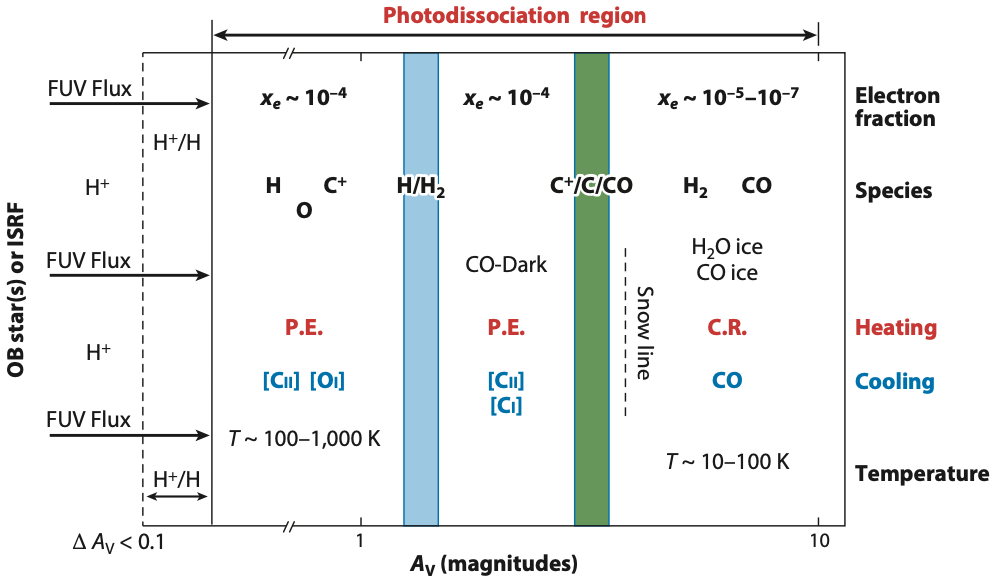
\includegraphics[width=.7\textwidth,keepaspectratio]{figures/PDRScheme_Wolfire2022fig2.png}
    \caption{Schematic of a photodissociation region as a function of visual extinction $A_V$. Reprinted from \textcite{Wolfire_2022}.}
\end{figure}
\subsection{The Horsehead Nebula}
\begin{figure}
    \centering
    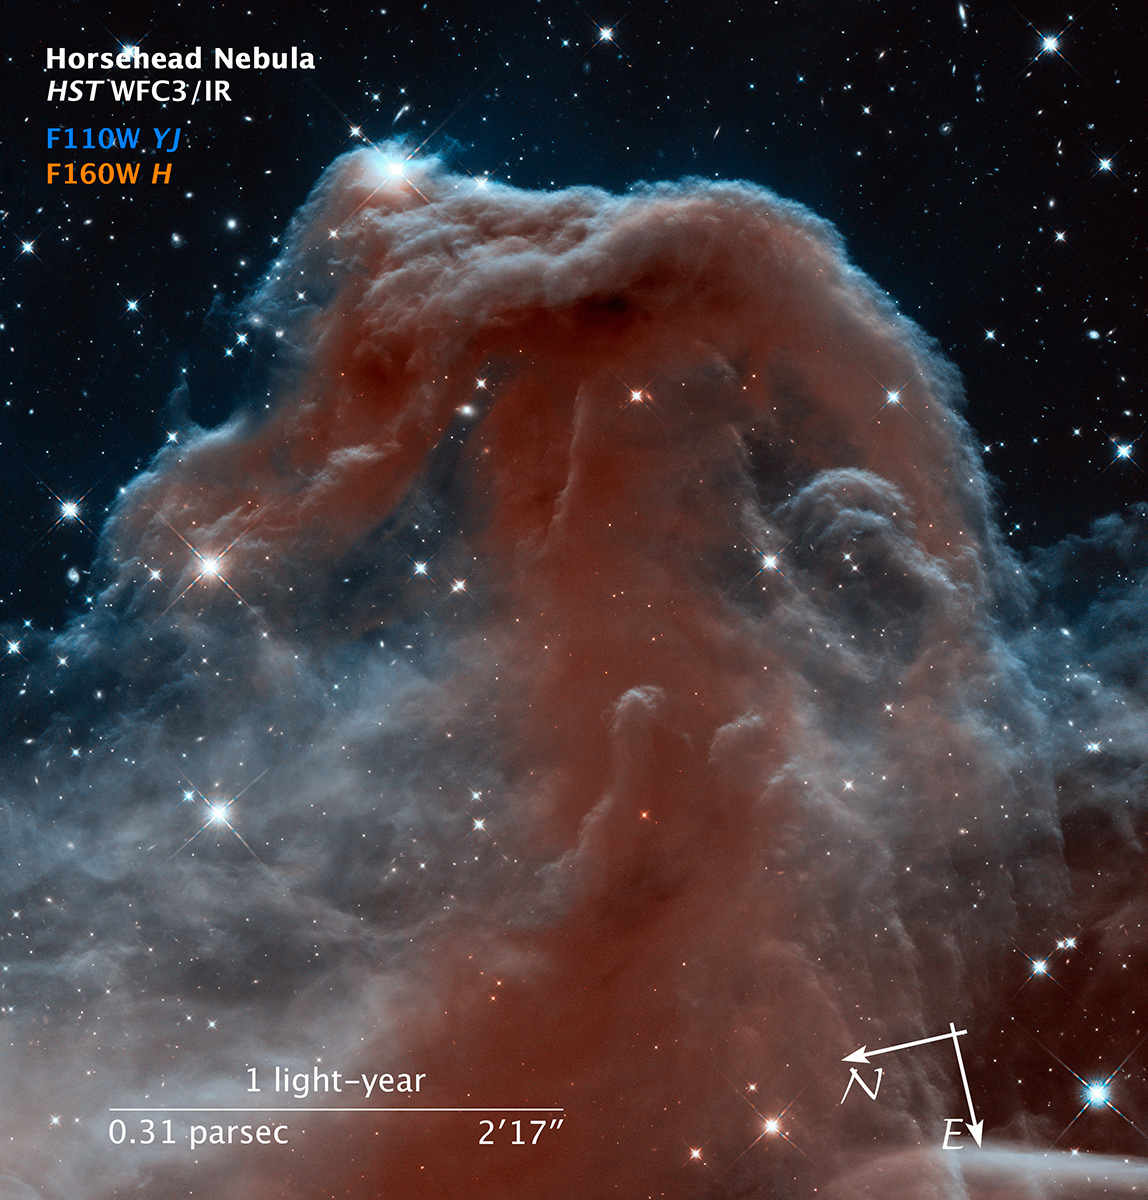
\includegraphics[width=.7\textwidth,keepaspectratio]{horsehead_hst.jpg}
    \caption{\href{https://hubblesite.org/contents/media/images/2013/12/3166-Image.html?keyword=Horsehead}{Horsehead Nebula captured by the Hubble Space Telescope (HST) in 2013.} The image was created from Hubble data from proposal \href{http://archive.stsci.edu/proposal_search.php?mission=hst&id=12812}{12812}. Illustration Credit: \href{http://www.nasa.gov/}{NASA}, \href{http://www.spacetelescope.org/}{ESA}, and Z. Levay (\href{http://www.stsci.edu/}{STScI})} 
\end{figure}

\begin{figure}
    \centering
    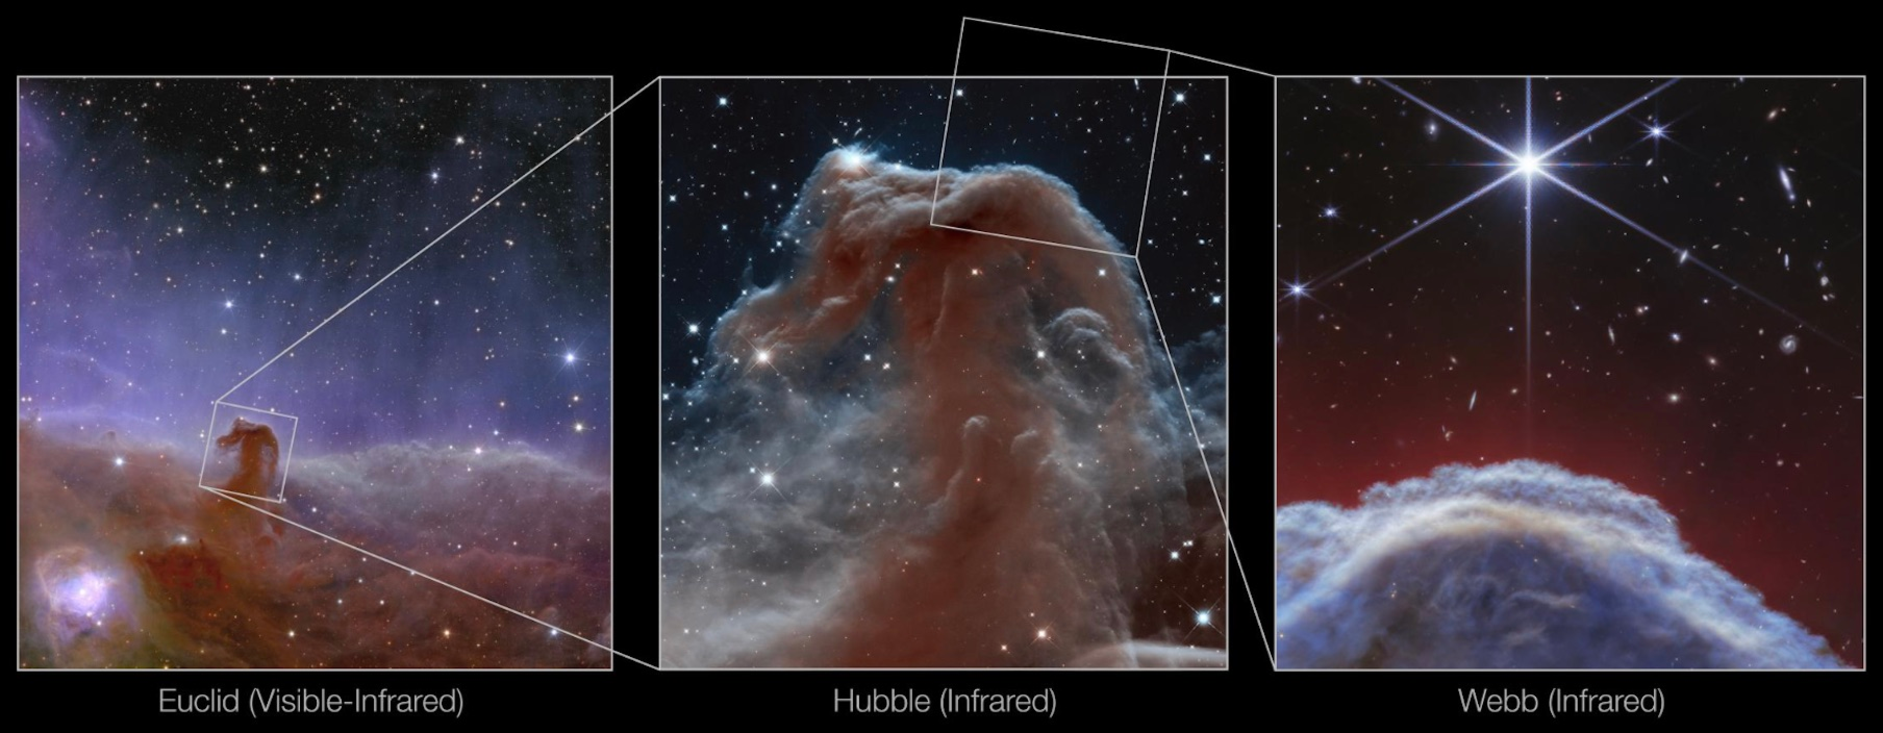
\includegraphics[width=\textwidth,keepaspectratio]{horsehead_zoomed.pdf}
    \caption{\href{https://www.esa.int/ESA_Multimedia/Images/2024/04/Webb_captures_iconic_Horsehead_Nebula_in_unprecedented_detail}{Three views of the Horsehead Nebula}. The first image (left) features the Horsehead Nebula as seen by ESA's Euclid telescope. The second image (middle) shows the NASA/ESA Hubble Space Telescope's infrared view of the Horsehead Nebula. The third image (right) features a new view of the Horsehead Nebula from the NASA/ESA/CSA James Webb Space Telescope's NIRCam (Near-InfraRed Camera) instrument.}
\end{figure}

In order to compare with observations, we need to convert the distance unit \unit{cm} used the in \mdpdr{} into the \unit{arcsec} unit used in observation,

\begin{equation}
    \alpha["] = \frac{d\,[\unit{pc}]}{400\,\unit{pc}} \frac{1\,\unit{arcsec}}{1\,\unit{rad}}\textbf{}
\end{equation}
where \qty{400}{pc} \parencite{Menten_2007, Schlafly_2014} is the distance to the horsehead nebula.

\section{Data}
In this report, my goal is to compare the observations of the Horsehead Nebula with the predictions of the \mdpdr{}. The observations were taken with \qt{Herschel}. The data were taken from the original paper \qt{add citation}.
% talk about Herschel
\begin{figure}
    \centering
    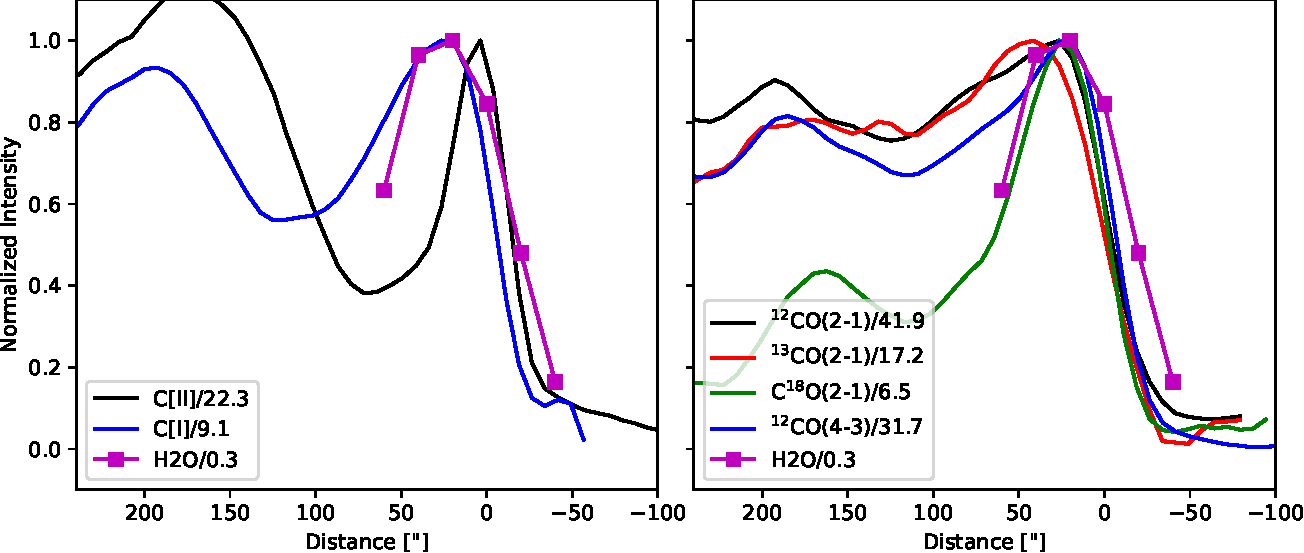
\includegraphics[width=\textwidth,keepaspectratio]{observed_lines.pdf}
    \caption{Observed line profiles of the Horsehead Nebula. Reproduced from \qt{cite the original paper}. The \ce{^{13}CO} lines has been removed due to bad weather condition during the observation.} \label{fig:observation}
\end{figure}


\section{Methods}
\subsection{The \mdpdr{}}
% first, ISM models in general
% caveats? PDR annual review section 5.5
A significant heterogeneity exists among the available PDR models, which differ in their geometry, physical and chemical structures, and model parameters. \qt{Röllig et al. (2007)} suggest that the choice of a spedific code should depend on the physical and chemical processes implemented in the code, as well as the characteristics of the emission source. 

In this project, I used the \mdpdr{} \parencite{LePetit_2006,Goicoechea_2007,Gonzalez_2008,LeBourlot_2012,Bron_thesis,Bron_2014,Bron_2016} to simulate the Horsehead Nebula. The \mdpdr{} models a stationary one-dimensional (1D), plane-parallel slab of gas and dust illuminated by an ultraviolet (UV) radiation field from one or both sides. At each iteration, the code solves the UV radiative transfer in both the continuum and lines, followed by the chemical balance, and finally the level populations and thermal balance. The code outputs the level populations, the gas temperature, and the chemical abundances as a function of the depth into the cloud, with optional output of the radiation field.

\subsubsection{Constant Pressure vs. Constant Density}

The density structure of the PDR model, such as constant density, constant pressure, or a density profile specified by the user, can have a significant influence on the simulation results. Observations reveal that there is a steep density gradient in the PDRs of the Horsehead Nebula \qt{(Habart et al. 2005; Guzmán et al. 2011) in C. Hernández-Vera 2023}. \qt{Hernández-Vera 2023} verified that the observations cannot be reproduced by a constant density model, yet neither by previously proposed density profile prescriptions. Later, observations by ALMA and Herschel suggest that the warm layer of PDRs is indeed isobaric with relatively large thermal pressures \qt{(Marconi et al. 1998; Goicoechea et al. 2016; Joblin et al. 2018; Wu et al. 2018; Bron et al. 2018; Maillard et al. 2021)}. For this reason, we use the constant pressure model in the \mdpdr{}.

The density structure of a photodissociation region model—whether constant density, constant pressure, or a user-defined density profile—can significantly influence the simulation results \qt{cite annual review}. Observations of the Horsehead Nebula reveal a steep density gradient in the PDRs \qt{{Habart 2005, Guzmán 2011, Hernández-Vera 2023}}. \qt{Hernández-Vera (2023)} showed that constant density models cannot reproduce observations, nor by previously proposed density profile prescriptions. Furthermore, recent observations from ALMA and Herschel indicate that the warm layer of PDRs is indeed isobaric, characterized by relatively high thermal pressures \qt{{Marconi 1998, Goicoechea 2016, Joblin 2018, Wu 2018, Bron 2018, Maillard 2021}}. For this reason, I use the constant pressure model in the \mdpdr{} for my study.

As shown in Fig.~\ref{fig:cmp_cstp_cstn}, I compare the cloud structure computed with constant pressure and constant density assumptions, illustrating the differences in the resulting PDR structures. In the constant pressure, the unphysical 

\begin{figure}
    \centering
    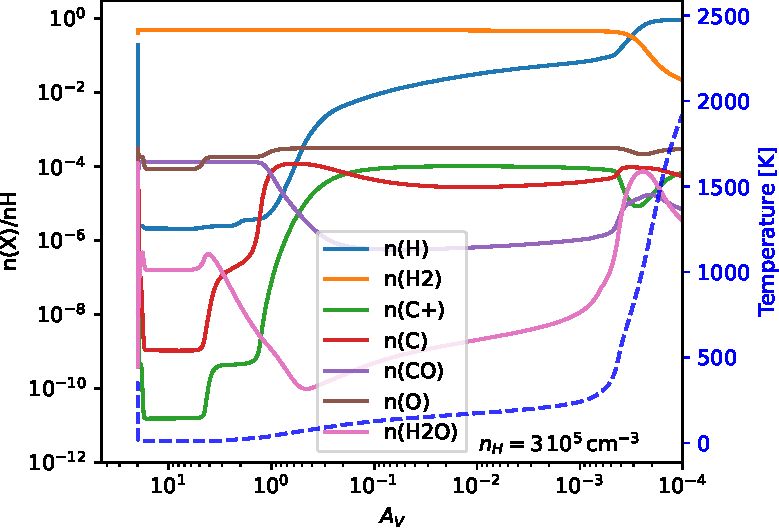
\includegraphics[width=.48\textwidth,keepaspectratio]{struct_nH3e5.pdf}
    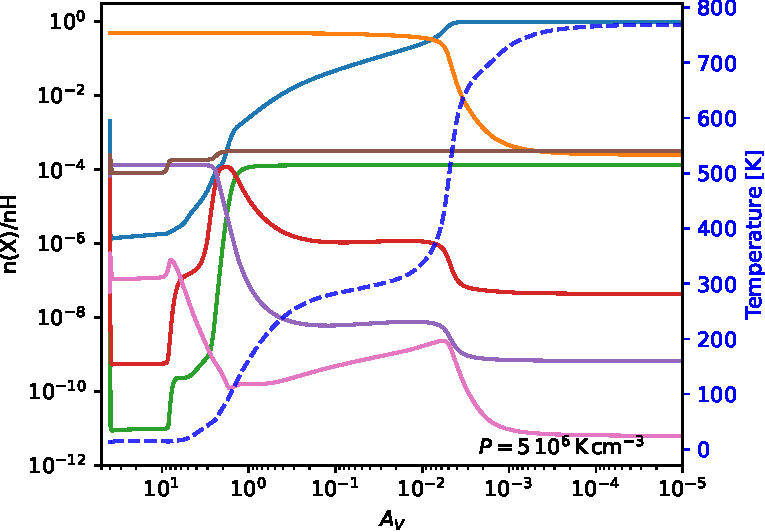
\includegraphics[width=.48\textwidth,keepaspectratio]{struct_P5e6.pdf}
    \caption{Comparison of the cloud structure computed with constant density (left) and constant pressure (right), with a shared legend displayed in the left plot.} \label{fig:cmp_cstp_cstn}
\end{figure}

\subsubsection{Models with Radiative Transfer of \ce{H2}}
\subsubsection{Models with Surface Chemistry}

\subsection{Geometry}
% \begin{wrapfigure}{r}{.32\textwidth}
%     \begin{center}
%         \includegraphics[width=.28\textwidth]{sphere_geometry_2LoS.pdf}
%     \end{center}
%     \caption{\qt{add a figure of the slab setup of the MeudonPDR code}Scheme of the plane-parallel geometry. Curvature exaggerated for clarity.} \label{fig:geometry}
% \end{wrapfigure}

\begin{figure}
    \centering
    \raisebox{-0.5\height}{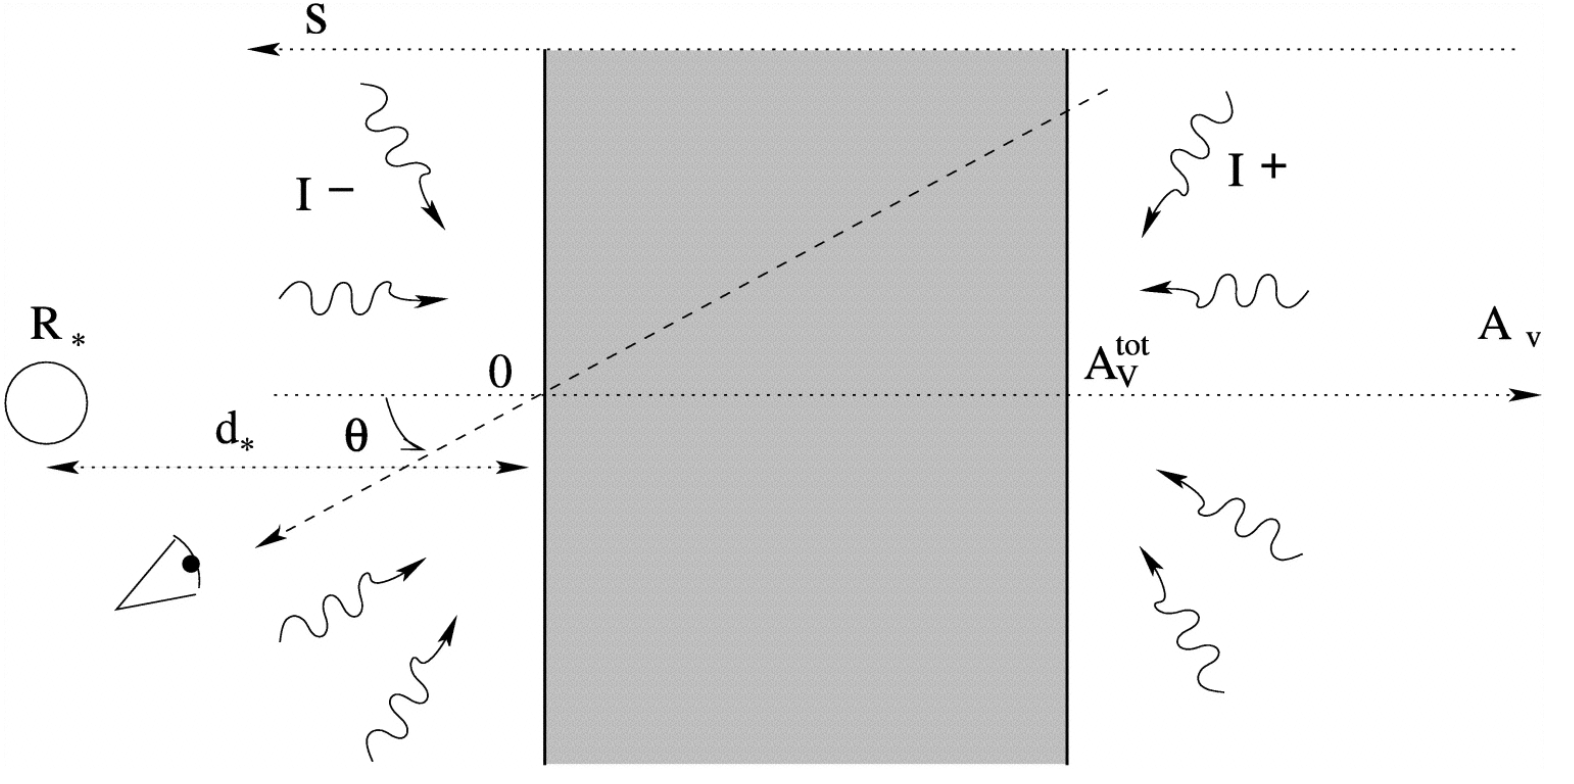
\includegraphics[width=.69\textwidth,keepaspectratio]{figures/slab_geometry.png}}
    \hfill
    \raisebox{-0.5\height}{\includegraphics[width=.24\textwidth,keepaspectratio]{figures/sphere_geometry_2LoS.pdf}}
    \caption{Left: scheme of the slab geometry of the \mdpdr{}. Reprinted from \textcite{LePetit_2006} Right: scheme of the plane-parallel geometry of the PDR wrapper.} \label{fig:geometry}
\end{figure}

In order to model the curvature of the cloud surface, we approximate the surface using plane-parallel geometry, as shown in Fig.~\ref{fig:geometry}.

More precisely, we consider the PDR region as the outermost shell embedded in a fictitious spherical cloud, whose radius $R$ will need to be determined by the user and is given as a parameter to the wrapper code.

A line of sight will be defined by an impact parameter $b$, which is the distance from the line-of-sight (LoS) to the center of the cloud. 

From the output of the \mdpdr{}, we have the number densities of levels as a function of the depth into the cloud, so we need to know the depth (i.e., the distance to the cloud surface) corresponding to each point along the LoS, we denote this quantity as $d$.

Using Pythagorean theorem, we can easily establish that
\begin{equation}
    d = R - \sqrt{s^2 + b^2} 
\end{equation}

\subsection{Column Density}

The wrapper code take as input:
\begin{itemize}
    \item the level number densities computed by the MeudonPDR code, as a function of the depth into the cloud, $n_X(d)$;
    \item the radius of the fictitious spherical cloud, $R$;
    \item the impact parameter of the LoS, $b$.
\end{itemize}
The algorithm goes as follow
\begin{enumerate}
    \item interpolate the level number density to enable the computation of the density at any valid given value of depth, $n_X(d) = f(d)$;
    \item compute the range of distances inside the PDR region along the LoS
    \begin{equation}
         s_{\max} = \sqrt{R^2 - b^2}, 
         s_{\min} = \left\{\begin{array}{ll}
            0  &  b > R - d_\mr{PDR} \\
            \sqrt{(R - d_\mr{PDR})^2 - b^2}  &  b < R - d_\mr{PDR}
         \end{array}\right.
         % \mr{maximum\ distance} = 2 s_{\max},
    \end{equation}
    \item convert the distance along the LoS to depth from the surface of the cloud, and compute the level number density
    \begin{equation}
        n_X(s) = f(R - \sqrt{s^2 + b^2});
    \end{equation}
    \item the column density for a given LoS with impact parameter $b$ is given by
    \begin{equation}
        N_X(b) = 2\int_{s_{\min}}^{s_{\max}} n_X(s') \dd{s'}.
    \end{equation}
\end{enumerate}

\subsection{Radiative transfer equation}
In the previous calculation of the column densities, we have made the assumption that all lines are optically thin; in fact, some of the lines can be optically thick, which explains the difference in the shape of the curve in observations for different lines in Fig~\ref{fig:observation}.

To account for line extinction inside the cloud, we need to solve the radiative transfer equation along the LoS \qt{cite see, for example, Eq (1.67) Rybicki?}:
\begin{equation}
    \fird[I_\nu]{s} = A_{ul} n_u\frac{h\nu}{4\pi}\phi(\nu) +  B_{ul} n_u\frac{h\nu}{4\pi}I_\nu \phi(\nu) -  B_{lu} n_l\frac{h\nu}{4\pi}I_\nu \phi(\nu), \label{eq:rte}
\end{equation}  
% or, in wavelength,
% \begin{equation}
%     \fird[I_\lambda]{s} = A_{ul} n_u\frac{h\nu}{4\pi}\phi(\lambda) +  B_{ul} n_u\frac{h\nu}{4\pi}I_\lambda \phi(\lambda) -  B_{lu} n_l\frac{h\nu}{4\pi}I_\lambda \phi(\lambda),
% \end{equation}
where $n_u$ and $n_l$ are the number densities of the upper and lower levels of the transition, respectively, $h$ is the Planck's constant, $\nu$ is the frequency of the transition, and $\phi(\nu)$ is the line profile. We assume that the emission and absorption profiles are the same and we neglect scattering \qt{justify?}. $A_{ul}, B_{ul}, B_{lu}$ are the Einstein coefficients for this transition, which are related by the Einstein relation \qt{references}
\begin{equation}
    B_{ul} = \frac{c^2}{2 h \nu_{ul}^3} A_{ul},\, g_l B_{lu} = g_u B_{ul},
\end{equation}
where $g_u$ and $g_l$ are the degeneracies of the upper and lower levels, respectively.

For consistency, we keep the same values for the Einstein coefficients as in the \mdpdr{}, which are taken from \qt{references?}.

In the PDR, turbulences are the dominant line broadening process \qt{references?  a bit more on line broadening in the intro?}, in which case the line profile $\phi(\nu)$ is a Gaussian profile in the form \qt{references}
\begin{equation}
    \phi(\nu) = \frac{1}{\sigma_\nu \sqrt{2 \pi}}\exp\left({-\frac{(\nu - \nu_0)^2}{2 \sigma_\nu^2}}\right),
\end{equation}
where
\begin{equation}
    \sigma_\nu = \frac{\sqrt{2}}{2}\Delta \nu_D,\,\Delta \nu_D = \frac{\nu_0}{c}\sqrt{\frac{2 k T}{m} + v_\mr{turb}^2}.
\end{equation}
% Or, equivalently, in wavelength
% \begin{equation}
%     \phi(\lambda) = \frac{1}{\sigma_\lambda \sqrt{2 \pi}}\exp\left({-\frac{(\lambda - \lambda_0)^2}{2 \sigma_\lambda^2}}\right),
% \end{equation}
% where
% \begin{equation}
%     \sigma_\lambda = \frac{\sqrt{2}}{2}\Delta \lambda_D,\,\Delta \lambda_D = \frac{\lambda_0}{c}\sqrt{\frac{2 k T}{m} + v_\mr{turb}^2}.
% \end{equation}
The turbulent velocity $v_\mr{turb}$ is a parameter in the \mdpdr{}, with a default value of \qty{2}{\km\per\second}. $T$ is the temperature, and $m$ is the mass of the line-emitting species. For the mass we use the same value as the \mdpdr{} (as defined in , taken from \href{https://www.sisweb.com/referenc/source/exactmas.htm}{\qt{Scientific Instrument Services (SIS) database? change name?}}

The line profile is normalized so that $\int_0^{\infty} \phi(\nu) \dd{\nu} = 1$. In practice, we truncate the line profile at $5\sigma$ \qt{add a figure to demonstrate that this is reasonable for the lines concerned?}, i.e., the normalization becomes
\begin{equation}
    \int_{\nu_0 - 5\sigma}^{\nu_0 + 5\sigma}\phi(\nu) \dd{\nu} = 1
\end{equation}

To solve the radiative transfer equation, we also need a background intensity $I_0$. For this we use the isotropic specific intensity on the observation side output by the \mdpdr{}, in the \mintinline{python}{_IncRadField.dat} file. 
\qt{add explanation that our implementation is only valid for isotropic radiation and explains why we couldn't implement a more generic background specific intensity.}

The external radiation field in the \mintinline{python}{_IncRadField.dat} file is in units of $\mr{erg\,cm^{-2}\,s^{-1}\,sr^{-1}\,\AA^{-1}}$, so we need to convert the specific intensity in to $\mr{erg\,cm^{-2}\,s^{-1}\,sr^{-1}\,Hz^{-1}}$,
\begin{equation}
    I_\nu |\dd{\nu}| = I_\lambda |\dd{\lambda}|  \Rightarrow I_\nu = I_\lambda \left|\frac{\dd{\lambda}}{\dd{\nu}}\right| = I_\lambda \frac{c}{\nu^2} = I_\lambda \frac{\lambda^2}{c}
\end{equation}
\begin{equation}
    \lambda = \frac{c}{\nu} \Rightarrow \dd{\lambda} = -\frac{c}{\nu^2}\dd{\nu} \Rightarrow \left|\frac{\dd{\lambda}}{\dd{\nu}}\right| = \frac{c}{\nu^2} = \frac{\lambda^2}{c}
\end{equation}

% In order to reduce numerical errors, we normalize Eq~\ref{eq:rte} as 
% \begin{equation}
    % \frac{4\pi}{h\nu}\fird[]{s}\left(\frac{I_\nu}{I_0}\right) = A_{ul} n_u\phi(\nu) +  B_{ul} n_u\frac{I_\nu}{I_0} \phi(\nu) -  B_{lu} n_l\frac{I_\nu}{I_0} \phi(\nu),
% \end{equation}

It is often more convenient to do a change of variable and integrate over optical depth
\begin{equation}
    \fird[I_\nu]{\tau_\nu} = S_\nu - I_\nu,
\end{equation}
with 
\begin{equation}
    \tau_\nu = \alpha_\nu \dd{s},\,S_\nu = \frac{j_\nu}{\alpha_\nu}
\end{equation}
\begin{equation}
     \alpha_\nu = \frac{h\nu}{4\pi} \phi(\nu)(B_{lu}n_l - B_{ul} n_u)
\end{equation}
\begin{equation}
    j_\nu = A_{ul} n_u \frac{h\nu}{4\pi} \phi(\nu)
\end{equation}

To test the solver, we first solve the radiative transfer with constant density profiles of both the lower and upper level, then the radiative transfer equation becomes
\begin{equation}
    \fird[I_\nu]{s} = c_1  + c_2 I_\nu, \label{eq:simple_rte}
\end{equation} 
with 
\begin{align*}
    &c_1 = A_{ul} n_u \frac{h\nu}{4\pi} \phi(\nu) = \mr{cst}\\
    &c_2 = \left(B_{ul} n_u - B_{lu} n_l\right) \frac{h\nu}{4\pi} \phi(\nu) = \mr{cst}.c
\end{align*}
The analytical solution is 
\begin{equation}
    I_\nu (s) = (I_0 + \frac{c_1}{c_2})e^{c_2s} - \frac{c_1}{c_2}.
\end{equation}

For example, if we consider the \ce{CO} transition from v = 0, J = 2 to v = 0, J = 1, with a constant density profile of $n_u = \qty{2}{\cm^{-3}}$, $n_l = \qty{2}{\cm^{-3}}$, $A_{ul} = 6.911 \times 10^{-7} s^{-1}$
\begin{itemize}
    \item $h\nu/4\pi = 4.86234284e-16 $
    \item $A_{ul} = 6.911e-07$
    \item $B_{ul} = 3825410.21021763$
    \item 
\end{itemize}

\subsection{Convolution}

\section{Results and Discussion}
\subsection{Cloud Surface Curvature}
\subsection{Line Profiles}

\section{Conclusions}

\newpage
\printbibliography

\end{document}